\documentclass[aspectratio=169,
hyperref={colorlinks,urlcolor=blue}
]{beamer}


%\usetheme{Pittsburgh}
\usetheme{default}
\usepackage{colortbl}%colored tables
%For using helvetica font:
\usepackage[scaled]{helvet}
\usepackage[T1]{fontenc}
\renewcommand\familydefault{\sfdefault}
\urlstyle{same} %sets the fonts for urls
\usepackage{pdfpages}
\usepackage{siunitx}
\usepackage{caption}
\usepackage{pifont}%for dings
\usepackage{pgfplots}%for 3d plotting
\pgfplotsset{compat = newest}
\usepackage{mathtools}%box in align env \Aboxed
\usepackage[american,smartlabels]{circuitikz}%for drawing circuits
\usepackage{multimedia}
\usepackage{animate}
\usepackage{xcolor}


\usetikzlibrary{arrows}
\usetikzlibrary {3d} 
\usetikzlibrary{decorations.markings, math}
\usetikzlibrary{intersections, pgfplots.fillbetween}
\usetikzlibrary {shapes.geometric} 


%\definecolor{myblue}{RGB}{5, 34, 150}
\definecolor{myblue2}{RGB}{5, 34, 150}
\definecolor{myblue}{RGB}{0,36,82}
\definecolor{myred}{RGB}{207, 2, 13}
\definecolor{mygreen}{RGB}{0, 158, 11}
\definecolor{myyellow}{RGB}{220,220,0}
\definecolor{qblue}{RGB}{0,36,82}
\definecolor{qgold}{RGB}{250,189,15}
\definecolor{qred}{RGB}{185,14,49}
\definecolor{cblue}{rgb}{0.13, 0.67, 0.8}
\definecolor{corange}{rgb}{0.8, 0.34, 0.0}
\definecolor{cpurple}{rgb}{0.54, 0.29, 0.42}

%%%%%%%%%%%% General settings
\setbeamercolor{frametitle}{fg=black}
\setbeamercolor{title}{fg=black}
\setbeamercolor{author}{fg=myblue2}

\beamertemplatenavigationsymbolsempty %no navigation controls at bottom of slides
%\setbeamertemplate{footline}[frame number]
\usefonttheme{professionalfonts} 
\setbeamerfont{title}{series=\bfseries,parent=structure}
\setbeamerfont{frametitle}{series=\bfseries,parent=structure}

%%%%%%%%%%%%Lists
\setbeamertemplate{itemize item}[circle] %{\color{myblue}$\circ$}
\setbeamertemplate{itemize subitem}{\color{myblue2}$\circ$}
\setbeamertemplate{itemize subsubitem}{\color{myblue2}$\cdot$}
\setbeamercolor{itemize item}{bg=myblue2,fg=myblue2}
\setbeamercolor{enumerate item}{bg=myblue2,fg=myblue2}
%%%%%%%%%%%%%%%%%%%%%%%%%%%%

%%%%%%%%%%%%Blocks
\setbeamertemplate{blocks}[rounded]
%Default block
\setbeamercolor{block title}{bg=myblue2, fg=white}
\setbeamercolor{block body}{bg=myblue2!10}
\setbeamerfont{block body}{size=\scriptsize}
\setbeamerfont{block title}{size=\scriptsize}
%Alert block
\setbeamercolor{block title alerted}{bg= myblue2, fg=white}
\setbeamercolor{block body alerted}{bg=myblue2!10}
\setbeamerfont{block body alerted}{size=\scriptsize}
\setbeamerfont{block title alerted}{size=\scriptsize}
%example block
\setbeamercolor{block title example}{bg=mygreen, fg=white}
\setbeamercolor{block body example}{bg=mygreen!10}
\setbeamerfont{block body example}{size=\scriptsize}
\setbeamerfont{block title example}{size=\scriptsize}
%%%%%%%%%%%%%%%%55


%%%%%%%%%%%%Figures and captions
\captionsetup{font=scriptsize,labelfont=scriptsize}
%\setbeamertemplate{caption}{\raggedright\insertcaption\par}
\newenvironment{capfig}[3]{\begin{figure}\includegraphics[width=#1\textwidth]{#2}\caption*{\textit{#3}}\end{figure}}{}

%\makeatother
%\setbeamertemplate{footline}
%{
%  \leavevmode%
%  \hbox{%
%  \begin{beamercolorbox}[wd=.4\paperwidth,ht=2.25ex,dp=1ex,center]{author in head/foot}%
%    \usebeamerfont{author in head/foot}\insertshortauthor
%  \end{beamercolorbox}%
%  \begin{beamercolorbox}[wd=.6\paperwidth,ht=2.25ex,dp=1ex,center]{title in head/foot}%
%    \usebeamerfont{title in head/foot}\insertshorttitle\hspace*{3em}
%    \insertframenumber{} / \inserttotalframenumber\hspace*{1ex}
%  \end{beamercolorbox}
%  }%
%  \vskip0pt%
%}
%\makeatletter

\makeatother
\setbeamertemplate{footline}
{
  \leavevmode%
  \hbox{%
\begin{beamercolorbox}[wd=.27\paperwidth,ht=2.25ex,dp=1ex,center]{author in head/foot}%
    \color{black}{\insertinstitute}
\end{beamercolorbox}
  \begin{beamercolorbox}[wd=.27\paperwidth,ht=2.25ex,dp=1ex,center]{author in head/foot}%
    \color{black}{\inserttitle}
  \end{beamercolorbox}%
  \begin{beamercolorbox}[wd=.27\paperwidth,ht=2.25ex,dp=1ex,center]{title in head/foot}%
    \color{black}{\insertshortauthor}
  \end{beamercolorbox}
  \begin{beamercolorbox}[wd=.27\paperwidth,ht=2.25ex,dp=1ex,center]{title in head/foot}%
    \hspace{.28\paperwidth}\color{black} \insertframenumber{} / \inserttotalframenumber\hspace*{1ex}
  \end{beamercolorbox}
  }%
  \vskip0pt%
}
\makeatletter

\setbeamertemplate{title page}
{
  \begin{tikzpicture}[remember picture,overlay]
    \def\barh{4}%15
  
    \draw[color=myblue2,line width=\barh] ([yshift=-0.5*\barh]current page.north west) -- ([yshift=-0.5*\barh,xshift=-0.67\paperwidth]current page.north east);
    \draw[color=myblue2,line width=\barh] ([yshift=-0.5*\barh,xshift=-0.67\paperwidth]current page.north east) -- ([yshift=-0.5*\barh,xshift=-0.34\paperwidth]current page.north east);
    \draw[color=myblue2,line width=\barh] ([yshift=-0.5*\barh,xshift=-0.34\paperwidth]current page.north east) -- ([yshift=-0.5*\barh]current page.north east); 
  
    \draw[color=myblue2,line width=\barh] ([yshift=0.5*\barh]current page.south west) -- ([yshift=0.5*\barh,xshift=-0.67\paperwidth]current page.south east);
    \draw[color=myblue2,line width=\barh] ([yshift=0.5*\barh,xshift=-0.67\paperwidth]current page.south east) -- ([yshift=0.5*\barh,xshift=-0.34\paperwidth]current page.south east);
    \draw[color=myblue2,line width=\barh] ([yshift=0.5*\barh,xshift=-0.34\paperwidth]current page.south east) -- ([yshift=0.5*\barh]current page.south east);
    %\node[left] at (current page.east) {
    %
\includegraphics[scale=0.1]{figures/coverpage}
    %};
  \end{tikzpicture}
  
  \usebeamerfont{title}\usebeamercolor[fg]{title}\inserttitle\par
  \usebeamerfont{subtitle}\usebeamercolor[fg]{subtitle}\insertsubtitle\par
  \vspace{2cm}
  \usebeamerfont{author}\usebeamercolor[fg]{author}\insertauthor\par
  \usebeamerfont{institute}\usebeamercolor[fg]{author}\insertinstitute\par
  \usebeamercolor[fg]{author}\par
  \usebeamercolor[fg]{titlegraphic}\inserttitlegraphic

} 

\setbeamertemplate{frametitle}{%
    \nointerlineskip%
        \par\hspace*{-\dimexpr0.5\paperwidth-0.5\textwidth}\textcolor{myblue2}{\rule{0.33\paperwidth}{6pt}}\textcolor{myblue2}{\rule{0.33\paperwidth}{6pt}}\textcolor{myblue2}{\rule{0.34\paperwidth}{6pt}} 
    \begin{beamercolorbox}[wd=\paperwidth,ht=0.75cm,dp=0.6ex]{frametitle}
        \hspace*{0.5cm}\strut\usebeamerfont{frametitle}\insertframetitle\strut
        %\hrule
    \end{beamercolorbox}%
    %%Line below:
%\par\hspace*{-\dimexpr0.5\paperwidth-0.5\textwidth}\textcolor{myblue}{\rule{\paperwidth}{0.4pt}}
     % <-- calculation of left margin width + rule
     %\textcolor{red}{\noindent\rule{\paperwidth}{2pt}}
}


%%%%%%%%%%%%Frame templates

%Slide with title
\newenvironment{titleframe}[1]
{\begin{frame}\frametitle{#1}\end{frame}}
{}

%Slide with title and itemize list:
\newenvironment{bulletframe}[1]
{\begin{frame}{#1} \itemize}
{\enditemize \end{frame}}

%Slide with two columns 50/50
\newenvironment{twocolframe}[3]
{\begin{frame}{#1}
 \begin{columns}[T]
 \column{0.5\textwidth}#2
 \column{0.5\textwidth}#3
 \end{columns}\end{frame}}{}

%Slide with two columns 60/40 <<<<<<<<<<<<<<<<<<<<<<  This one!
\newenvironment{twocolframesf}[3]
{\begin{frame}{#1}
 \begin{columns}[T]
 \column{0.6\textwidth}#2
 \column{0.4\textwidth}#3
 \end{columns}\end{frame}}{}
 
%Slide with two columns 70/30
\newenvironment{twocolframest}[3]
{\begin{frame}{#1}
 \begin{columns}[T] 
 \column{0.7\textwidth}#2
 \column{0.3\textwidth}#3
 \end{columns}\end{frame}}{} 
 
%Slide with two columns 40/60
\newenvironment{twocolframefs}[3]
{\begin{frame}{#1}
 \begin{columns}[T] 
 \column{0.4\textwidth}#2
 \column{0.6\textwidth}#3
 \end{columns}\end{frame}}{}
 
%Slide with two columns 70/30
\newenvironment{twocolframets}[3]
{\begin{frame}{#1}
 \begin{columns}[T] 
 \column{0.3\textwidth}#2
 \column{0.7\textwidth}#3
 \end{columns}\end{frame}}{} 

 
%Colloquium speaker (title, abstract, picture file, speaker name)
\newenvironment{colloquium}[5]
{
\begin{frame}{Colloquium: Friday 1:30pm in Stirling A}
\begin{columns}[T] 
 \column{0.8\textwidth}
 \textbf{#1}\\
 #2
 \column{0.2\textwidth}
 \capfig{#3}{#4}{#5}
 \end{columns}
\end{frame}
}
{} 

%%%%%%%%%%%%%Set Hyperref colors


\hypersetup{
  colorlinks=true,
  linkcolor=blue,    
  urlcolor=blue,     
  citecolor=blue      
}
%%%%%%%%%%%%%TOC bolding
\setbeamerfont{section in toc}{series=\bfseries}



%Frames:
% \twocolframesf 60/40 (fs, st, ts) 
% \titleframe
% bulletframe


%%%%%%%%%%%%%%%%%%%%%%%%%
%%%%%% START OF PRESENTATION %%%%%%
%%%%%%%%%%%%%%%%%%%%%%%%%

\title{Waves}
\subject{Wave Properties, Descriptions and Phenomena}
\subtitle{Building Models to Describe our World}


\begin{document}

%%%%%%%%%%%%%%%%%%%%%%%%%
%%%%%% Title slide %%%%%%
%%%%%%%%%%%%%%%%%%%%%%%%%
\chaptertitle{Waves}
\begin{frame}
\titlepage
\thispagestyle{empty}
\end{frame}

%%%%%%%%%%%%%%%%%%%%%%%%%%%%%%%%
%%Advertisements and such %%%%%%
%%%%%%%%%%%%%%%%%%%%%%%%%%%%%%%%

\twocolframe{Outline}
  {\tableofcontents[sections={1,2}, subsectionstyle=show/show]\thispagestyle{empty}}
  {\tableofcontents[sections={3}, subsectionstyle=show/show]}

%%%%%%%%%%%%%%




%%%%%%%%%%%%%%%%%%%%%%%%%%%%%%%%
\section{Properties of a Wave}
\label{sec:propertiesofawave}
\title{Properties of a Wave}
%%%%%%%%%%%%%%%


\begin{frame}
\titlepage
\thispagestyle{empty}
\end{frame}



%%%%%%%%%%%%%%
\subsection{Speed of a wave}
\label{subsec:speedofawave}
\twocolframe{Speed of a wave}
{
\begin{itemize}
\item Depends only on the medium through which it propagates (e.g. speed of sound does not depend on what is making the sound).
\item If the particles in the medium are heavier, they have more inertia and they oscillate about their equilibrium slower $\rightarrow$ Waves are slower in denser media.
\item If the medium is ``stiffer'' (the force trying to restore the particles to equilibrium is larger), they will oscillate faster $\rightarrow$ Waves are faster in stiffer media.


\end{itemize}
}
{
\begin{itemize}
\item For waves on a rope with tension  and linear mass density:
\begin{align*}
v=\sqrt{\frac{F_T}{\mu}}
\end{align*}
\end{itemize}
\begin{block}{Analogous to a simple harmonic
oscillator}
\vspace{-0.25cm}
\begin{align*}
\omega =\sqrt{\frac{k}{m}}=2\pi f
\end{align*}
\vspace{-0.5cm}
\begin{itemize}
\item For a stiffer spring constant, the
oscillator has a higher frequency.
\item For a larger mass, the oscillator
has a lower frequency.
\end{itemize}

\end{block}
}


%%%%%%%%%%%%%%%%%%%%%%%%%%%%%%%%

%%%%%%%%%%%%%%%%%%%%%%%%%%%%%%%%

\subsection{Reflection}
\label{subsec:reflection}
\twocolframe{Pulse reflection}
{
Fixed end, reflection inverted:
\begin{center}
\begin{animateinline}[autoplay,loop]{5} % 5 fps, same as 0.2 s transduration
\multiframe{40}{i=1+1}{
\begin{tikzpicture}[scale=1]
\tikzmath{
\L=5;
\h=2;
\Am=1.5;%height
\As=0.1*\L;%width
\Ax=-1.1*\L+\i*0.05*1.1*\L;
\Axi=\Ax-0.5*\As;
\Axf=\Ax+0.5*\As;
}
\useasboundingbox (-\L,-\h) rectangle (0.4,\h);
\scalebox{1}{
\fill (0,-\h) rectangle (0.5,\h);
\begin{scope}
\clip (-\L,-\Am) rectangle (0,\Am);
\ifthenelse{\i<20}
{
\draw[color=brown,line width=3] (-\L,0)-- (\Axi,0)-- (\Ax,\Am) --(\Axf,0)-- (0,0);
}
{
\draw[color=brown,line width=3] (0,0)-- (-\Axi,0)-- (-\Ax,-\Am)-- (-\Axf,0)-- (-\L,0);
}
\end{scope}
}
\end{tikzpicture}
}
\end{animateinline}
\captionof*{figure}{\textit{Think of rope exerting upwards force on wall, so wall exerts downwards force on rope, which starts a negative pulse going to the left}}
\end{center}

}
{
Open end, reflection in the same direction
\begin{center}
\begin{animateinline}[autoplay,loop]{5} % 5 fps, same as 0.2 s transduration
\multiframe{40}{i=1+1}{
\begin{tikzpicture}[scale=1]
\tikzmath{
\L=5;
\h=2;
\Am=1.5;%height
\As=0.1*\L;%width
\Ax=-1.1*\L+\i*0.05*1.1*\L;
\Axi=\Ax-0.5*\As;
\Axf=\Ax+0.5*\As;
}
\useasboundingbox (-\L,-\h) rectangle (0.4,\h);
\scalebox{1}{
\fill (0,-\h) rectangle (0.5,\h);
\begin{scope}
\clip (-\L,-\Am) rectangle (0.1,\Am);
\ifthenelse{\i<20}
{
\draw[color=brown,line width=3] (-\L,0)-- (\Axi,0)-- (\Ax,\Am) --(\Axf,0)-- (0.1,0);
}
{
\draw[color=brown,line width=3] (0.1,0)-- (-\Axi,0)-- (-\Ax,\Am)-- (-\Axf,0)-- (-\L,0);
}
\end{scope}
}
\end{tikzpicture}
}
\end{animateinline}
\captionof*{figure}{\textit{The end of the rope moves up when pulse arrives, which starts a positive pulse going to the left}}
\end{center}
}



%%%%%%%%%%%%%%%%%%%%%%%%%%%%%%%%



%%%%%%%%%%%%%%%%%%%%%%%%%%%%%%%%
\subsection{Transmission}
\label{subsec:transmission}
\begin{frame}{Reflection and transmission}
\begin{itemize}
\item When a pulse changes medium, part of it is reflected and part is transmitted.

\begin{center}
\begin{animateinline}[autoplay,loop]{5} % 5 fps, same as 0.2 s transduration
\multiframe{40}{i=1+1}{
\begin{tikzpicture}[scale=1]
\tikzmath{
%\i=10;
\L=5;
\h=2;
\Am=1.5;%height
\As=0.1*\L;%width
\Ax=-1.1*\L+\i*0.05*1.1*\L;
\Axi=\Ax-0.5*\As;
\Axf=\Ax+0.5*\As;
}
\useasboundingbox (-\L,-\Am) rectangle (\L,\Am);

\scalebox{1}{
\ifthenelse{\i<20}
{
\draw[color=brown,line width=1] (-\L,0)-- (\Axi,0)-- (\Ax,\Am) --(\Axf,0)-- (0,0);
\draw[color=brown,line width=3] (0,0) -- (\L,0);
}
{
%\draw[color=brown,line width=1] (-\L,0)-- (0,0);
\draw[color=brown,line width=1] (0,0)-- (-\Axi,0)-- (-\Ax,-0.2*\Am) --(-\Axf,0)-- (-\L,0);
\draw[color=brown,line width=3] (0,0) --(\Axi,0)-- (\Ax,0.6*\Am) -- (\Axf,0) --  (\L,0);
}
}


\end{tikzpicture}
}
\end{animateinline}
\captionof*{figure}{\textit{When the second section is heavier, it reflect the same as a fixed end.}}
\end{center}

\item The amplitude (and sign) of the reflected part is related to the reflection coefficient:
\begin{align*}
R=\frac{\sqrt\mu_1-\sqrt\mu_2}{\sqrt\mu_1+\sqrt\mu_2}
\end{align*}

\end{itemize}

\end{frame}


%%%%%%%%%%%%%%%%%%%%%%%%%%%%%%%%
\begin{frame}{Reflection and transmission}
\begin{itemize}
\item When a pulse changes medium, part of it is reflected and part is transmitted.

\begin{center}
\begin{animateinline}[autoplay,loop]{5} % 5 fps, same as 0.2 s transduration
\multiframe{40}{i=1+1}{
\begin{tikzpicture}[scale=1]
\tikzmath{
%\i=10;
\L=5;
\h=2;
\Am=1.5;%height
\As=0.1*\L;%width
\Ax=-1.1*\L+\i*0.05*1.1*\L;
\Axi=\Ax-0.5*\As;
\Axf=\Ax+0.5*\As;
}
\useasboundingbox (-\L,-\Am) rectangle (\L,\Am);

\scalebox{1}{
\ifthenelse{\i<20}
{
\draw[color=brown,line width=3] (-\L,0)-- (\Axi,0)-- (\Ax,\Am) --(\Axf,0)-- (0,0);
\draw[color=brown,line width=1] (0,0) -- (\L,0);
}
{
%\draw[color=brown,line width=1] (-\L,0)-- (0,0);
\draw[color=brown,line width=3] (0,0)-- (-\Axi,0)-- (-\Ax,0.2*\Am) --(-\Axf,0)-- (-\L,0);
\draw[color=brown,line width=1] (0,0) --(\Axi,0)-- (\Ax,0.6*\Am) -- (\Axf,0) --  (\L,0);
}
}


\end{tikzpicture}
}
\end{animateinline}
\captionof*{figure}{\textit{When the second section is lighter, it reflect the same as an open end.}}
\end{center}

\item The amplitude (and sign) of the reflected part is related to the reflection coefficient:
\begin{align*}
R=\frac{\sqrt\mu_1-\sqrt\mu_2}{\sqrt\mu_1+\sqrt\mu_2}
\end{align*}

\end{itemize}

\end{frame}


%%%%%%%%%%%%%%%%%%%%%%%%%%%%%%%%










%%%%%%%%%%%%%%%%%%%%%%%%%%%%%%%%

\section{Describing a Wave}
\label{sec:describingawave}
\title{Describing a Wave}


\begin{frame}
\titlepage
\thispagestyle{empty}
\end{frame}

%%%%%%%%%%%%%%%%%%%%%%%%%%%%%%%%%%%%
\subsection{How to describe a wave}
\label{subsec:howtodescribeawave}
\twocolframesf{How to describe a wave}
{
\begin{itemize}
\item A wave is a series of pulses. The easiest type of wave to describe is one where the pulses are generated by a periodic mechanism (e.g. the end of the rope moving up and down at constant frequency). 
\item If the end of the rope moves like a simple harmonic oscillator, then you obtain a sine wave. 
\item[$\rightarrow$] To fully describe a wave, we need to describe the position of each point in the medium as a function of time.
\item[$\rightarrow$] $D(x,t)$, distance of the point at position $x$ from its equilibrium position at time $t$.
\item[$\rightarrow$] $D(x,t)$ depends on \textbf{position and time}.

\end{itemize}

}
{
\vspace{-1cm}
\begin{center}
\begin{animateinline}[autoplay,loop]{10} % 5 fps, same as 0.2 s transduration
\multiframe{40}{i=1+1}{
\begin{tikzpicture}[scale=1]
\tikzmath{
\L=4.5;
\h=2;
\Ax=1.5;
\om=2;
\xmax=pi/\om/2;
\phas=\i*2*pi/40;
\xmaxs=(pi/2+\phas)/\om;
\xs=pi/\om;
\ys=\Ax*sin( (\om*\xs-\phas)/pi*180 );
}

\scalebox{1}{
\coordinate (P) at (\xmax,\Ax);
\coordinate (P2) at (\xmaxs,\Ax);
\coordinate (P3) at (\xs,\ys);

 \draw[line width=0.5, color=black!50] (0,-\h) grid (\L,\h);
 \draw[-latex,line width=1] (0,0) -- +(1.1*\L,0) node[below]{$x$};
 \draw[-latex,line width=1] (0,0) -- +(0,1.1*\h) node[left]{$D$};
 
 \draw[dashed,color=myred] (\L,\Ax) -- (0,\Ax) node[left]{$A$};
 \draw[dashed,color=myred] (\L,-\Ax) -- (0,-\Ax) node[left]{$-A$};
 
 \draw[trig format=rad, line width=2] plot[ domain=0:\L, variable=\x, samples=100] ({\x},{\Ax*sin(\om*\x)});
 \draw[trig format=rad, line width=2, color=myblue!40] plot[ domain=0:\L, variable=\x, samples=100] ({\x},{\Ax*sin(\om*\x-\phas)});
 
 \draw[dashed,color=myblue!40,line width=1.5] (\xs,-\Ax) -- (\xs,\Ax);
 \fill[color=myblue!40] (P3) circle(6pt);
 \fill[color=myred] (P) circle(2pt); 
 \fill[color=myred] (P2) circle(2pt); 
 
 %\draw[color=myred,-latex, line width=2] (P) -- (P2) node[midway,above]{$v$};
 %Legend:
 \draw[line width=2] (0.1*\L,1.2*\h) -- +(0.5,0) node[right]{$t=0$};
 \draw[line width=2, color=myblue!40] (0.5*\L,1.2*\h) -- +(0.5,0) node[right]{$t$};
}
\end{tikzpicture}
}
\end{animateinline}
\captionof*{figure}{\textit{A sine wave propagating at constant speed through a medium. Each point in the medium executes SHM.}}
\end{center}
At time $t=0$, we have:
\begin{align*}
D(x,t=0)=A\sin\left(\frac{2\pi}{\lambda}x\right)
\end{align*}
}



%%%%%%%%%%%%%%%%%%%%%%%%%%%%%%%%


%%%%%%%%%%%%%%%%%%%%%%%%%%%%%%%%
\subsection{Describing a traveling wave}
\label{subsec:describingatravelingwave}
\twocolframesf{Traveling wave description}
{
\begin{itemize}
\item At time $t=0$, we can describe the displacement of each point in the medium by:
\begin{align*}
D(x,t=0)=A\sin\left(\frac{2\pi}{\lambda}x\right)
\end{align*}
\item At time $t$, the point at position $x$ will have the same displacement as the point at $x-vt$ had at $t=0$:
\begin{align*}
D(x,t) &= D(x-vt,t=0)\\
&=A\sin\left (\frac{2\pi}{\lambda}(x-vt)\right)
\end{align*}
\end{itemize}

}
{
\begin{center}

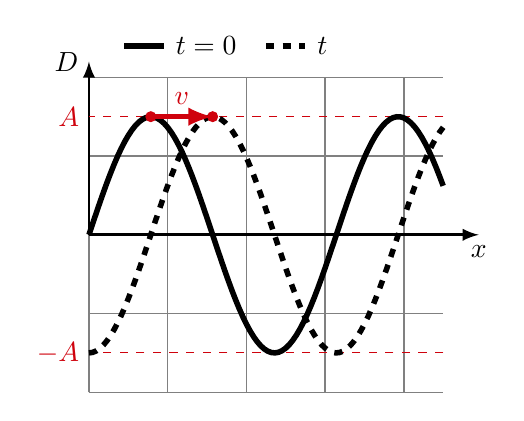
\begin{tikzpicture}[scale=1]
\tikzmath{
\L=4.5;
\h=2;
\Ax=1.5;
\om=2;
\phas=0;
\xmax=pi/\om/2;
\shif=1.5*pi/3;
\xmaxs=(pi/2+\shif)/\om;
}

\scalebox{1}{
\coordinate (P) at (\xmax,\Ax);
\coordinate (P2) at (\xmaxs,\Ax);
 \draw[line width=0.5, color=black!50] (0,-\h) grid (\L,\h);
 \draw[-latex,line width=1] (0,0) -- +(1.1*\L,0) node[below]{$x$};
 \draw[-latex,line width=1] (0,0) -- +(0,1.1*\h) node[left]{$D$};
 
 \draw[dashed,color=myred] (\L,\Ax) -- (0,\Ax) node[left]{$A$};
 \draw[dashed,color=myred] (\L,-\Ax) -- (0,-\Ax) node[left]{$-A$};
 
 \draw[trig format=rad, line width=2] plot[ domain=0:\L, variable=\x, samples=100] ({\x},{\Ax*sin(\om*\x-\phas)});
 \draw[trig format=rad, line width=2, dashed] plot[ domain=0:\L, variable=\x, samples=100] ({\x},{\Ax*sin(\om*\x-\phas-\shif)});
 
 \fill[color=myred] (P) circle(2pt); 
 \fill[color=myred] (P2) circle(2pt); 
 \draw[color=myred,-latex, line width=2] (P) -- (P2) node[midway,above]{$v$};
 
 \draw[line width=2] (0.1*\L,1.2*\h) -- +(0.5,0) node[right]{$t=0$};
 \draw[line width=2, dashed] (0.5*\L,1.2*\h) -- +(0.5,0) node[right]{$t$};
}
\end{tikzpicture}

\captionof*{figure}{\textit{When a sine wave propagates through the medium, each point in the medium moves back and forth about some equilibrium position.}}
\end{center}
}



%%%%%%%%%%%%%%%%%%%%%%%%%%%%%%%%
\subsubsection{Wavelength and period}
\label{subsubsec:wavelengthandperiod}
\begin{frame}{Description of a wave using wavelength and period}
\begin{align*}
D(x,t) =A\sin\left (\frac{2\pi}{\lambda}(x-vt)\right)
\end{align*}
\begin{itemize}
\item The speed of the wave, $v$, is related to its wavelength, $\lambda$, and period, $T$:
\begin{align*}
v&=\frac{\lambda}{T}\\
\therefore D(x,t) &=A\sin\left (\frac{2\pi}{\lambda}x-\frac{2\pi}{T}t\right)
\end{align*}
\end{itemize}
\end{frame}


%%%%%%%%%%%%%%%%%%%%%%%%%%%%%%%%
\subsubsection{Phase and wave number}
\label{subsubsec:phaseandwavenumber}
\begin{frame}{General description, phase, wave number}
\begin{itemize}
\item In general, the displacement need not be $D=0$ at $x=0$ and time $t=0$. The wave can be ``shifted'' to the left or to the right by a ``phase'', $\phi$:
\begin{align*}
 D(x,t) &=A\sin\left (\frac{2\pi}{\lambda}x-\frac{2\pi}{T}t +\phi\right)
\end{align*}
\item Clean up the notation to get rid of the $2\pi$:
\begin{align*}
 D(x,t) &=A\sin\left (kx-\omega t +\phi\right)
\end{align*}
by introducing wave number, $k$, and angular frequency, $\omega$:
\begin{align*}
k&=\frac{2\pi}{\lambda}\\
\omega&=\frac{2\pi}{T}=2\pi f\\
\end{align*}
\end{itemize}
\vspace{-0.5cm}
Wave number and angular frequency are directly related to wavelength and period/frequency, simply a cleaner version without the $2\pi$.
\end{frame}


%%%%%%%%%%%%%%%%%%%%%%%%%%%%%%%%




%%%%%%%%%%%%%%%%%%%%%%%%%%%%%%%%
\subsection{SHM review}
\label{subsec:shmreview}
\twocolframesf{Recall: simple harmonic motion}
{
\begin{itemize}
\item Any system described by the following undergoes Simple Harmonic Motion:
\begin{align*}
\frac{d^2x}{dt^2}&=-\omega^2 x\\
\therefore x(t)&=A\cos(\omega t +\phi)
\end{align*}
\item SHM arises from physics where there is a \textit{restoring} force that is \textit{linearly} proportional to displacement. For example, $F=-kx$ .
\item All of the physics is contained in $\omega$, the angular frequency of the motion:
\begin{align*}
\omega = \sqrt{\frac{k}{m}}\quad,\quad\omega =  \sqrt{\frac{g}{L}}
\end{align*} 
\end{itemize}
}
{
\begin{center}
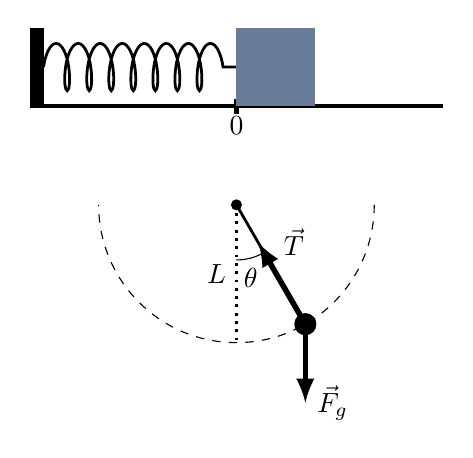
\begin{tikzpicture}[scale=1]
\tikzmath{
\L=1.75;
\dx=0.75*\L;
\off=0.5;
\h=1;
\th=30;
}
\scalebox{1}{

\draw[line width=1.5pt] (-1.5*\L,0) -- (1.5*\L,0) ;
\draw[line width=1.5pt] (0,-0.1) -- (0,0.1);
\node[below] at (0,0) {$0$};

\fill (-1.5*\L,0) rectangle (-1.4*\L,\h);
\draw[decoration={aspect=0.3, segment length=2.8mm, amplitude=3mm,coil},decorate,line width=1pt] (-1.4*\L,\h/2) -- (0,\h/2);
%\draw [latex-latex] (-1.4*\L,\h) -- (0,\h) node[midway,above]{$L_0$};
\fill[myblue!60] (0,0) rectangle (\h,\h);

\begin{scope}[shift={(0,-1.25*\h)}]
\coordinate (P) at (270+\th:\L);
\fill (0,0) circle (2pt);
\fill (P) circle (4pt);
\draw[line width=1] (0,0) -- (P) ;
\draw[dotted,line width=1] (0,0) -- +(0,-\L) node[midway, left]{$L$};
\draw[dashed] (\L,0) arc (0:-180:\L);

\draw[-latex, line width=2] (P) -- +(90+\th:1.2) node[right=5pt]{$\vec T$};
\draw[-latex, line width=2] (P) -- +(0,-1) node[right]{$\vec F_g$};

\draw (0,-0.7) arc (270:270+\th:0.7) node[midway,below]{$\theta$};

\end{scope}
}
\end{tikzpicture}
\captionof*{figure}{\textit{A spring-mass system or a simple pendulum are examples of systems that undergo simple harmonic motion.}}
\end{center}

}


%%%%%%%%%%%%%%%%%%%%%%%%%%%%%%%%
\begin{frame}{A sine wave and SHM}
\begin{center}

\begin{animateinline}[autoplay,loop]{10} % 5 fps, same as 0.2 s transduration

\multiframe{24}{i=1+1}{

\begin{tikzpicture}[scale=1]
\tikzmath{
\h=2;
\L=12;
\wl=\L/2;%wavelength
\om=2*pi/\wl;%effective frequency
\phas=2*pi/24*\i;
\Ax=0.5;
}

\useasboundingbox (0,-2*\Ax) rectangle (\L,\h+0.2);
\scalebox{1}{

\fill (0,\h) rectangle +(\L,0.2);
\draw[trig format=rad, line width=2] plot[ domain=0:\L, variable=\x, samples=100] ({\x},{\Ax*cos(\om*\x-\phas)});

\foreach \xl in  {0.1,0.2,0.3,0.4,0.5,0.6,0.7,0.8,0.9}{
  \tikzmath{
    \xp=\xl*\L;
    \yp=\Ax*cos((\om*\xp-\phas)*180/pi);%needs to be in degrees...
    \lcy=(\h-\yp);
  }
  \coordinate (P) at (\xp,\yp);
  \draw[decoration={aspect=0.3, segment length=\lcy mm, amplitude=3mm,coil},decorate,line width=1pt] (\xp,\h) -- (P);
  \fill (P) circle (4pt);
}
  
}
\end{tikzpicture}
}
\end{animateinline}

\captionof*{figure}{\textit{A sine wave going through a medium corresponds to particles in the medium being displaced in SHM.}}
\end{center}
\end{frame}


%%%%%%%%%%%%%%%%%%%%%%%%%%%%%%%%
\subsection{The wave equation (in 1D)}
\label{subsec:thewaveequationin1d}
\begin{frame}{The wave equation (1D)}
\begin{itemize}
\item Similarly, any physics model that gives ``the wave equation'':
\begin{align*}
\frac{\partial^2D}{\partial x^2}=\frac{1}{v^2}\frac{\partial^2D}{\partial t^2}
\end{align*}
corresponds to the propagation of a wave.
\item A possible mathematical description/solution is:
\begin{align*}
D(x,t) &=A\sin\left (kx-\omega t +\phi\right)
\end{align*}
Where:
\begin{itemize}
\item $A$ is the amplitude of the wave and depends on what is creating the wave (e.g. how high you shake the end of a rope).
\item $\omega$ and $k$ (or equivalently $T$ and $\lambda$) are related by:
\begin{align*}
\frac{\omega}{k}=\frac{\lambda}{T}=v
\end{align*}
\end{itemize}
Only one of $\omega$ and $k$ is independent, since the speed, $v$, depends on the medium and not what creates the wave. 
\end{itemize}
\end{frame}


%%%%%%%%%%%%%%%%%%%%%%%%%%%%%%%%



%%%%%%%%%%%%%%%%%%%%%%%%%%%%%%%%
\subsubsection{Solutions}
\label{subsubsec:solutions}
\begin{frame}{Wave equation solutions, linear superposition}
\begin{itemize}
\item An infinite number of functions, $D(x,t)$, can solve the wave equation:
\begin{align*}
\frac{\partial^2D}{\partial x^2}=\frac{1}{v^2}\frac{\partial^2D}{\partial t^2}
\end{align*}
For example:
\begin{align*}
D_1(x,t) &=A_1\sin\left (k_1x-\omega_1 t +\phi_1\right)\\
D_2(x,t) &=A_1\cos\left (k_2x-\omega_2 t +\phi_2\right)\\
\dots&
\end{align*}
\item You can also show that any linear combination of these functions (or other possible solutions) will also satisfy the wave equation:
\begin{align*}
D_3(x,t)=a_1D_1(x,t)+a_2D_2(x,t)
\end{align*}
\end{itemize}
\end{frame}


%%%%%%%%%%%%%%%%%%%%%%%%%%%%%%%%
\subsection{Pulse on a tense rope}
\label{subsec:pulseonatenserope}
\twocolframesf{A physics model for a pulse on a rope with tension}
{
We can model the vertical acceleration of a small piece of rope of length $dx$:
\only<1>{
}
\only<2>{
\begin{itemize}
\item This leads to the wave equation in the form:
\begin{align*}
\frac{\partial^2D}{\partial x^2}=\frac{\mu}{F_T}\frac{\partial^2D}{\partial t^2}
\end{align*}
\item Compare with the wave equation:
\begin{align*}
\frac{\partial^2D}{\partial x^2}=\frac{1}{v^2}\frac{\partial^2D}{\partial t^2}
\end{align*}
and identify that:
\begin{align*}
v=\sqrt{\frac{F_T}{\mu}}
\end{align*}
\end{itemize}

}
}
{
\begin{center}
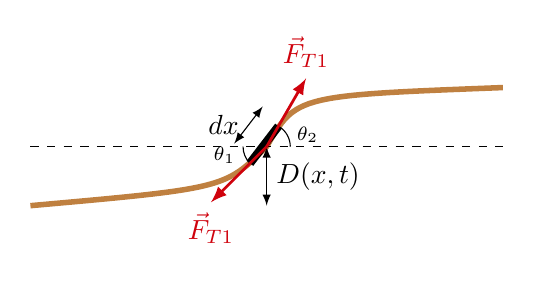
\begin{tikzpicture}[scale=1]
\tikzmath{
\L=3;
\h=0.75;
\th1=45;
\th2=60;
}
\scalebox{1}{
\coordinate (P1) at (-\L,-\h);
\coordinate (P2) at (0,0);
\coordinate (P3) at (\L,\h);
\coordinate (C1) at ($(P2)+(180+\th1:0.25*\L)$);
\coordinate (C2) at ($(P2)+(\th2:0.25*\L)$);
\draw[line width=2, color=brown] (P1) .. controls (C1) .. (P2) .. controls (C2) .. (P3);

\draw (0.3,0) arc(0:\th2:0.3) node[midway,right]{\scriptsize$\theta_2$};
\draw (-0.3,0) arc(180:180+\th1:0.3) node[midway,left]{\scriptsize$\theta_1$};

\draw[line width=3] ($(P2)+(180+\th1:0.1*\L)$) -- ($(P2)+(\th2:0.1*\L)$);
\draw[latex-latex] ($(P2)+(180+\th1:0.1*\L)+(-0.2,0.25)$) -- ($(P2)+(\th2:0.1*\L)+(-0.2,0.25)$) node[midway][left]{$dx$};
\draw[latex-latex] (0,0) -- (0,-\h) node[midway,right]{$D(x,t)$};
\draw[dashed] (-\L,0) -- (\L,0);

\draw[-latex, line width=1, color=myred] (P2) -- +(180+\th1:1) node[below]{$\vec F_{T1}$};
\draw[-latex, line width=1, color=myred] (P2) -- +(\th2:1) node[above]{$\vec F_{T1}$};
}
\end{tikzpicture}
\captionof*{figure}{\textit{Modeling a pulse on a rope.}}
\end{center}

}

%%%%%%%%%%%%%%%%%%%%%%%%%%%%%%%%


\section{Energy Transport and Phenomena of Waves}
\label{sec:energytransportandphenomenaofwaves}
\title{Energy Transport and Phenomena of Waves}


\begin{frame}
\titlepage
\thispagestyle{empty}
\end{frame}



%%%%%%%%%%%%%%%%%%%%%%%%%%%%%%%%
\subsection{Energy transport of a wave}
\label{subsec:energytransportofawave}
\begin{frame}{Energy transport in a wave}
\begin{center}

\begin{animateinline}[autoplay,loop]{10} % 5 fps, same as 0.2 s transduration

\multiframe{24}{i=1+1}{

\begin{tikzpicture}[scale=1]
\tikzmath{
\h=2;
\L=12;
\wl=\L/2;%wavelength
\om=2*pi/\wl;%effective frequency
\phas=2*pi/24*\i;
\Ax=0.5;
}

\useasboundingbox (0,-2*\Ax) rectangle (\L,\h+0.2);
\scalebox{1}{

\fill (0,\h) rectangle +(\L,0.2);
\draw[trig format=rad, line width=2] plot[ domain=0:\L, variable=\x, samples=100] ({\x},{\Ax*cos(\om*\x-\phas)});

\foreach \xl in  {0.1,0.2,0.3,0.4,0.5,0.6,0.7,0.8,0.9}{
  \tikzmath{
    \xp=\xl*\L;
    \yp=\Ax*cos((\om*\xp-\phas)*180/pi);%needs to be in degrees...
    \lcy=(\h-\yp);
  }
  \coordinate (P) at (\xp,\yp);
  \draw[decoration={aspect=0.3, segment length=\lcy mm, amplitude=3mm,coil},decorate,line width=1pt] (\xp,\h) -- (P);
  \fill (P) circle (4pt);
}
  
}
\end{tikzpicture}
}
\end{animateinline}

\captionof*{figure}{\textit{A sine wave going propagating through a medium modeled as a collection of SHOs.}}
\end{center}
We can think of each point in the medium as a simple harmonic oscillator that moves up and down with the \textbf{same period/frequency and the same amplitude} as the wave traveling through the medium.
\end{frame}


%%%%%%%%%%%%%%%%%%%%%%%%%%%%%%%%



%%%%%%%%%%%%%%%%%%%%%%%%%%%%%%%%
\subsubsection{1D wave}
\label{subsubsec:1dwave}
\begin{frame}{Energy transport in a 1D wave}
\begin{itemize}
\item Energy of one oscillator:
\begin{align*}
E=\frac{1}{2}\omega^2 m A^2
\end{align*}
\item If the oscillator is a small mass element on a rope:
\begin{align*}
dm=\mu dx
\end{align*}
    with energy:     
\begin{align*}
dE=\frac{1}{2}\omega^2dmA^2=\frac{1}{2}\omega^2\mu dx A^2
\end{align*}
\item The energy ``contained'' in 1 wavelength is the sum of the energies of the oscillators in one wavelength:
\begin{align*}
E_\lambda=\int dE=\int_0^\lambda \frac{1}{2}\omega^2\mu dx A^2 = \frac{1}{2}\omega^2\mu A^2\lambda
\end{align*}
\end{itemize}

\end{frame}


%%%%%%%%%%%%%%%%%%%%%%%%%%%%%%%%

\begin{frame}{Power transport in a 1D wave}
\begin{itemize}
\item Power is the rate at which energy is being expended:
\begin{align*}
P=\frac{\Delta E}{\Delta t}
\end{align*}
\item Over one period of the wave, $T$, you need to expend the energy ``contained'' in one wavelength:
\begin{align*}
P=\frac{\frac{1}{2}\omega^2\mu A^2\lambda}{T}=\frac{1}{2}\omega^2\mu A^2 v
\end{align*}
since:     
\begin{align*}
v=\frac{\lambda}{T}
\end{align*}
\item This is the power that you have to put in to sustain the wave (and the rate at which energy is ``received'' at the other end).
\end{itemize}

\end{frame}

%%%%%%%%%%%%%%%%%%%%%%%%%%%%%%%%
\subsubsection{3D wave}
\label{subsubsec:3dwave}
\twocolframesf{Energy transport in a 3D spherical wave}
{
\begin{itemize}
\item A spherical sound wave corresponds to successive shells of air contracting and expanding (longitudinal wave). 
\item We can model each shell as a simple harmonic oscillator with mass $dm$ and spring constant $k_s$.
\item If each shell has the same thickness, $dr$, then the outer shells have higher mass:
\begin{align*}
dm=\rho dV = \rho 4\pi r^2 dr
\end{align*}
\item The energy in a shell is then given by:
\begin{align*}
dE=\frac{1}{2}k_sA^2=\frac{1}{2}\omega^2 dm A^2 = 2\pi\rho\omega^2A^2r^2dr
\end{align*}
\end{itemize}
}
{
\begin{center}

\begin{animateinline}[autoplay,loop]{15} % 5 fps, same as 0.2 s transduration
\multiframe{15}{i=1+1}{

\begin{tikzpicture}[scale=1]
\tikzmath{
\R=2;
\dr=0.25;
}
\useasboundingbox (-1.25*\R,-1.25*\R) rectangle (1.25*\R,1.25*\R);
\scalebox{1}{

\foreach \nf in {5,4,3,2,1}{
  \tikzmath{
    \r=\nf*0.2*\R;
    \imax=3*(\nf-1)+1;
    \imin=3*(\nf)-1;
  }
  \ifthenelse{\i=\imin}{  %compress a shell
    \fill[color=black!50] (0,0) circle (\r+\dr-0.075);
    \fill[color=white] (0,0) circle (\r-0.075);
  }
  {
  \begin{scope}
    \fill[color=black!50] (0,0) circle (\r+\dr);
    \fill[color=white] (0,0) circle (\r);
  \end{scope}
  }
  \ifthenelse{\i=\imax}{ %expand a shell
    \fill[color=black!50] (0,0) circle (\r+\dr+0.075);
    \fill[color=white] (0,0) circle (\r+0.075);
  }
  {
  \begin{scope}
    \fill[color=black!50] (0,0) circle (\r+\dr);
    \fill[color=white] (0,0) circle (\r);
  \end{scope}
  }


}


}
\end{tikzpicture}
}
\end{animateinline}
\captionof*{figure}{\textit{A spherical longitudinal wave propagating through successive concentric shells, each with thickness, $dr$.}}
\end{center}

}


%%%%%%%%%%%%%%%%%%%%%%%%%%%%%%%%
\begin{frame}{Energy transport in a 3D spherical wave}
\begin{itemize}
\item Energy in one shell:
\begin{align*}
dE= 2\pi\rho\omega^2A^2r^2dr
\end{align*}
\item Power (rate at which energy moves from one shell to the next):
\begin{align*}
P=\frac{dE}{dt}=\frac{dE}{dr}\frac{dr}{dt}=\frac{dE}{dr}v= 2\pi\rho\omega^2A^2r^2v
\end{align*}
\end{itemize}
\end{frame}


%%%%%%%%%%%%%%%%%%%%%%%%%%%%%%%%


%%%%%%%%%%%%%%%%%%%%%%%%%%%%%%%%
\subsection{Intesnity of a wave}
\label{subsec:intensityofawave}
\begin{frame}{Intensity of a wave}
\begin{itemize}
\item The intensity of a spherical wave is the power that it delivers into a specific area (for example, the area of your ear for a sound wave).
\item At some distance $r$ from the source, the total power per unit area is given by:
\begin{align*}
I=\frac{\text{Power}}{\text{Area}}=\frac{P}{4\pi r^2}=\frac{1}{2}\rho \omega^2A^2v\propto \frac{1}{r^2}
\end{align*}
\item Your ear is sensitive to the intensity of a sound wave (as your house is sensitive to the intensity of an earthquake). \item It is sensitive to the rate at which energy is delivered to your ear drum. 
\item Since the amplitude goes down as $1/r$, the intensity of the wave goes down as $/r^2$.  
\end{itemize}
\end{frame}

%%%%%%%%%%%%%%%%%%%%%%%%%%%%%%%%




%%%%%%%%%%%%%%%%%%%%%%%%%%%%%%%%
\subsection{Superposition}
\label{subsec:superposition}
\begin{frame}{Superposition of waves}
Recall that many functions can solve the wave equation:
\begin{align*}
\frac{\partial^2D}{\partial x^2}=\frac{1}{v^2}\frac{\partial^2D}{\partial t^2}
\end{align*}
In particular, if $D_1(x,t)$ and $D_2(x,t)$ are solutions, so is any linear combination thereof:
\begin{align*}
D_3(x,t)=a_1D_1(x,t)+a_2D_2(x,t)
\end{align*}
\end{frame}



%%%%%%%%%%%%%%%%%%%%%%%%%%%%%%%%
\subsubsection{Fourier's Theorem}
\label{subsubsec:fourierstheorem}
\twocolframesf{Superposition and Fourier's theorem}
{
\begin{itemize}
\item If you have several mechanisms generating waves, the resultant waves is the sum of each individual wave.
\item \textbf{Fourier's theorem}: Any periodic function can always be expressed as a sum of sinusoidal functions. $\rightarrow$ Thus, we can study sinusoidal waves without any loss in generality.
\end{itemize}
}
{
\vspace{-1cm}
\begin{center}
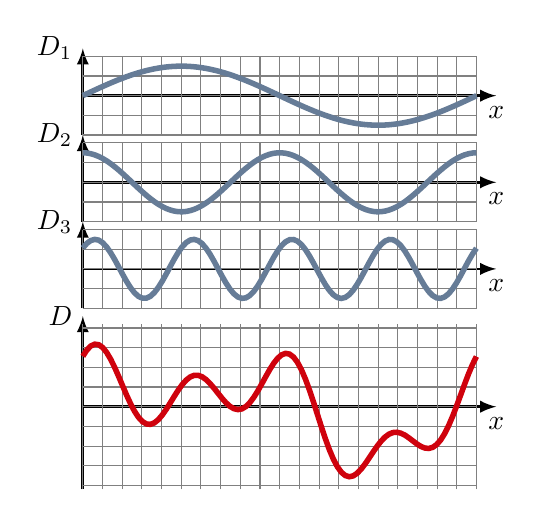
\begin{tikzpicture}[scale=1]
\tikzmath{
\L=5;
\h=0.5;
\Ax1=0.75*\h;
\wl1=\L;%wavelength
\om1=2*pi/\wl1;%effective frequency
\Ax2=0.75*\h;
\wl2=\L/2;%wavelength
\om2=2*pi/\wl2;%effective frequency
\Ax3=0.75*\h;
\wl3=\L/4;%wavelength
\om3=2*pi/\wl3;%effective frequency
}
\scalebox{1}{

\draw[-latex,line width=1] (0,-\h) -- (0,1.2*\h) node[left]{$D_1$};
\draw[-latex,line width=1] (0,0) -- (1.05*\L,0) node[below]{$x$};

\draw[color=black!50] (0,-\h) grid[step=0.25] (\L,\h);
\draw[trig format=rad, line width=2,color=myblue!60] plot[ domain=0:\L, variable=\x, samples=100] ({\x},{\Ax1*sin(\om1*\x)});

\begin{scope}[shift={(0,-2.2*\h)}]
\draw[-latex,line width=1] (0,-\h) -- (0,1.2*\h) node[left]{$D_2$};
\draw[-latex,line width=1] (0,0) -- (1.05*\L,0) node[below]{$x$};
\draw[color=black!50] (0,-\h) grid[step=0.25] (\L,\h);
\draw[trig format=rad, line width=2,color=myblue!60] plot[ domain=0:\L, variable=\x, samples=100] ({\x},{\Ax2*sin(\om2*\x+pi/2)});
\end{scope}

\begin{scope}[shift={(0,-4.4*\h)}]
\draw[-latex,line width=1] (0,-\h) -- (0,1.2*\h) node[left]{$D_3$};
\draw[-latex,line width=1] (0,0) -- (1.05*\L,0) node[below]{$x$};
\draw[color=black!50] (0,-\h) grid[step=0.25] (\L,\h);
\draw[trig format=rad, line width=2,color=myblue!60] plot[ domain=0:\L, variable=\x, samples=100] ({\x},{\Ax3*sin(\om3*\x+pi/4)});
\end{scope}

\begin{scope}[shift={(0,-7.9*\h)}]
\draw[-latex,line width=1] (0,-2.1*\h) -- (0,2.3*\h) node[left]{$D$};
\draw[-latex,line width=1] (0,0) -- (1.05*\L,0) node[below]{$x$};
\draw[color=black!50] (0,-2.1*\h) grid[step=0.25] (\L,2.1*\h);
\draw[trig format=rad, line width=2,color=myred] plot[ domain=0:\L, variable=\x, samples=100] ({\x},{\Ax1*sin(\om1*\x)+ \Ax2*sin(\om2*\x+pi/2)+\Ax3*sin(\om3*\x+pi/4)});
\end{scope}

}
\end{tikzpicture}
\captionof*{figure}{\textit{The bottom wave, $D$, is the superposition of the 3 sinusoidal waves, $D=D_1+D_2+D_3$.}}
\end{center}
}


%%%%%%%%%%%%%%%%%%%%%%%%%%%%%%%%
\subsubsection{Fourier decomposition}
\label{subsubsec:fourierdecomposition}
\twocolframesf{Example: Fourrier decomposition of a square wave}
{
\begin{itemize}
\item Even a square wave can be modeled as the sum of sine waves:
\begin{align*}
f(x)=\frac{4}{\pi}\sum_{n=1,3,5,\dots}^\infty \frac{1}{n}\sin\left( \frac{n\pi x}{L} \right)
\end{align*}
where the square wave has wavelength $2L$ and amplitude of 1. 
\item[$\rightarrow$] Without loss of generality, we can worry only about sine waves!
\end{itemize}
}
{
\vspace{-1cm}
\begin{center}
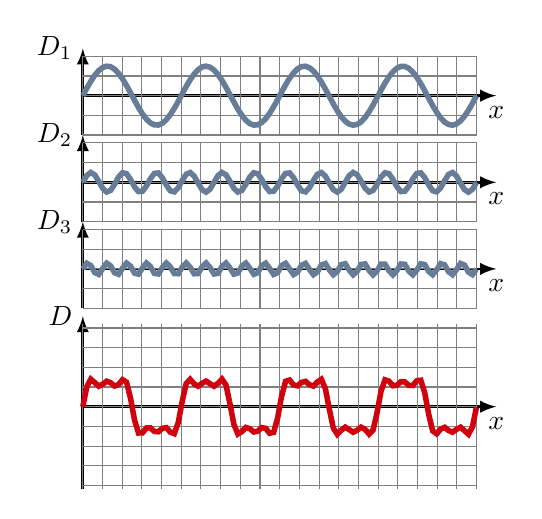
\begin{tikzpicture}[scale=1]
\tikzmath{
\L=5;
\h=0.5;
\Ax1=0.75*\h;
\wl1=\L/4;%wavelength
\om1=2*pi/\wl1;%effective frequency
\Ax2=\Ax1/3;
\om2=3*\om1;%effective frequency
\Ax3=\Ax1/5;
\om3=5*\om1;%effective frequency
}
\scalebox{1}{

\draw[-latex,line width=1] (0,-\h) -- (0,1.2*\h) node[left]{$D_1$};
\draw[-latex,line width=1] (0,0) -- (1.05*\L,0) node[below]{$x$};

\draw[color=black!50] (0,-\h) grid[step=0.25] (\L,\h);
\draw[trig format=rad, line width=2,color=myblue!60] plot[ domain=0:\L, variable=\x, samples=100] ({\x},{\Ax1*sin(\om1*\x)});

\begin{scope}[shift={(0,-2.2*\h)}]
\draw[-latex,line width=1] (0,-\h) -- (0,1.2*\h) node[left]{$D_2$};
\draw[-latex,line width=1] (0,0) -- (1.05*\L,0) node[below]{$x$};
\draw[color=black!50] (0,-\h) grid[step=0.25] (\L,\h);
\draw[trig format=rad, line width=2,color=myblue!60] plot[ domain=0:\L, variable=\x, samples=100] ({\x},{\Ax2*sin(\om2*\x)});
\end{scope}

\begin{scope}[shift={(0,-4.4*\h)}]
\draw[-latex,line width=1] (0,-\h) -- (0,1.2*\h) node[left]{$D_3$};
\draw[-latex,line width=1] (0,0) -- (1.05*\L,0) node[below]{$x$};
\draw[color=black!50] (0,-\h) grid[step=0.25] (\L,\h);
\draw[trig format=rad, line width=2,color=myblue!60] plot[ domain=0:\L, variable=\x, samples=100] ({\x},{\Ax3*sin(\om3*\x)});
\end{scope}

\begin{scope}[shift={(0,-7.9*\h)}]
\draw[-latex,line width=1] (0,-2.1*\h) -- (0,2.3*\h) node[left]{$D$};
\draw[-latex,line width=1] (0,0) -- (1.05*\L,0) node[below]{$x$};
\draw[color=black!50] (0,-2.1*\h) grid[step=0.25] (\L,2.1*\h);
\draw[trig format=rad, line width=2,color=myred] plot[ domain=0:\L, variable=\x, samples=100] ({\x},{\Ax1*sin(\om1*\x)+ \Ax2*sin(\om2*\x)+\Ax3*sin(\om3*\x)});
\end{scope}

}
\end{tikzpicture}
\captionof*{figure}{\textit{Adding sine waves to make a square wave. This converges in the limit of an infinite sum.}}
\end{center}
}



%%%%%%%%%%%%%%%%%%%%%%%%%%%%%%%%
\subsection{Interference}
\label{subsec:interference}
\twocolframesf{Interference}
{
\begin{itemize}
\item Sometimes, the waves that sum together ``interfere'' in ``constructive'' or ``destructive'' ways.
\item To get a complete interference, you need waves of the same frequency/wavelength to interfere.
\end{itemize}
}
{
\vspace{-1cm}
\begin{center}

\begin{animateinline}[autoplay,loop]{10} % 5 fps, same as 0.2 s transduration

\multiframe{24}{i=1+1}{

\begin{tikzpicture}[scale=1]
\tikzmath{
\L=5;
\h=0.7;
\Ax1=0.75*\h;
\wl1=\L/4;%wavelength
\om1=2*pi/\wl1;%effective frequency
\Ax2=\Ax1;
\om2=\om1;%effective frequency
\phas=-2*pi/24*\i;
}
\scalebox{1}{

\draw[-latex,line width=1] (0,-\h) -- (0,1.2*\h) node[left]{$D_1$};
\draw[-latex,line width=1] (0,0) -- (1.05*\L,0) node[below]{$x$};

\draw[color=black!50] (0,-\h) grid[step=0.25] (\L,\h);
\draw[trig format=rad, line width=2,color=myblue!60] plot[ domain=0:\L, variable=\x, samples=100] ({\x},{\Ax1*sin(\om1*\x+\phas)});

\begin{scope}[shift={(0,-2.2*\h)}]
\draw[-latex,line width=1] (0,-\h) -- (0,1.2*\h) node[left]{$D_2$};
\draw[-latex,line width=1] (0,0) -- (1.05*\L,0) node[below]{$x$};
\draw[color=black!50] (0,-\h) grid[step=0.25] (\L,\h);
\draw[trig format=rad, line width=2,color=myblue!60] plot[ domain=0:\L, variable=\x, samples=100] ({\x},{\Ax2*sin(\om2*\x+\phas)});
\end{scope}

\begin{scope}[shift={(0,-5.9*\h)}]
\draw[-latex,line width=1] (0,-2.1*\h) -- (0,2.3*\h) node[left]{$D$};
\draw[-latex,line width=1] (0,0) -- (1.05*\L,0) node[below]{$x$};
\draw[color=black!50] (0,-2.1*\h) grid[step=0.25] (\L,2.1*\h);
\draw[trig format=rad, line width=2,color=myred] plot[ domain=0:\L, variable=\x, samples=100] ({\x},{\Ax1*sin(\om1*\x+\phas)+ \Ax2*sin(\om2*\x+\phas)});
\end{scope}

}
\end{tikzpicture}
}
\end{animateinline}
\captionof*{figure}{\textit{Constructive interference between two identical waves in phase.}}
\end{center}
}



%%%%%%%%%%%%%%%%%%%%%%%%%%%%%%%%
\twocolframesf{Interference}
{
\begin{itemize}
\item Sometimes, the waves that sum together ``interfere'' in ``constructive” or ``destructive'' ways.
\item To get a complete interference, you need waves of the same frequency/wavelength to interfere
\end{itemize}
}
{
\vspace{-1cm}
\begin{center}

\begin{animateinline}[autoplay,loop]{10} % 5 fps, same as 0.2 s transduration

\multiframe{24}{i=1+1}{

\begin{tikzpicture}[scale=1]
\tikzmath{
\L=5;
\h=0.7;
\Ax1=0.75*\h;
\wl1=\L/4;%wavelength
\om1=2*pi/\wl1;%effective frequency
\Ax2=\Ax1;
\om2=\om1;%effective frequency
\phas=-2*pi/24*\i;
}
\scalebox{1}{

\draw[-latex,line width=1] (0,-\h) -- (0,1.2*\h) node[left]{$D_1$};
\draw[-latex,line width=1] (0,0) -- (1.05*\L,0) node[below]{$x$};

\draw[color=black!50] (0,-\h) grid[step=0.25] (\L,\h);
\draw[trig format=rad, line width=2,color=myblue!60] plot[ domain=0:\L, variable=\x, samples=100] ({\x},{\Ax1*sin(\om1*\x+\phas)});

\begin{scope}[shift={(0,-2.2*\h)}]
\draw[-latex,line width=1] (0,-\h) -- (0,1.2*\h) node[left]{$D_2$};
\draw[-latex,line width=1] (0,0) -- (1.05*\L,0) node[below]{$x$};
\draw[color=black!50] (0,-\h) grid[step=0.25] (\L,\h);
\draw[trig format=rad, line width=2,color=myblue!60] plot[ domain=0:\L, variable=\x, samples=100] ({\x},{\Ax2*sin(\om2*\x+\phas+pi)});
\end{scope}

\begin{scope}[shift={(0,-5.9*\h)}]
\draw[-latex,line width=1] (0,-2.1*\h) -- (0,2.3*\h) node[left]{$D$};
\draw[-latex,line width=1] (0,0) -- (1.05*\L,0) node[below]{$x$};
\draw[color=black!50] (0,-2.1*\h) grid[step=0.25] (\L,2.1*\h);
\draw[trig format=rad, line width=2,color=myred] plot[ domain=0:\L, variable=\x, samples=100] ({\x},{\Ax1*sin(\om1*\x+\phas)+ \Ax2*sin(\om2*\x+\phas+pi)});
\end{scope}

}
\end{tikzpicture}
}
\end{animateinline}
\captionof*{figure}{\textit{Destructive interference between two identical waves out of phase.}}
\end{center}
}


%%%%%%%%%%%%%%%%%%%%%%%%%%%%%%%%
\subsubsection{Double-slit}
\label{subsubsec:doubleslit}
\twocolframe{Interference, double-slit}
{
\begin{center}
\begin{tikzpicture}[scale=1]
\tikzmath{
\d=0.75;
\h=1.25;
\w=0.25;
\gap=0.25;
}
\scalebox{1}{

\fill[color=myblue!60] (-\w/2,-\d/2) rectangle (\w/2,\d/2);
\fill[color=myblue!60] (-\w/2,\d/2+\gap) rectangle (\w/2,\d/2+\gap+\h);
\fill[color=myblue!60] (-\w/2,-\d/2-\gap) rectangle (\w/2,-\d/2-\gap-\h);

\foreach \n in {1,...,10}{
\draw[color=myred] (-\w/2-\n*\w,-\d/2-\gap-\h) -- (-\w/2-\n*\w,\d/2+\gap+\h);
}

\foreach \n in {1,...,5}{
\draw[color=myred] (\w/2,\d/2+\gap/2+\n*\w) arc (90:-90:\n*\w);
\draw[color=myred] (\w/2,-\d/2-\gap/2+\n*\w) arc (90:-90:\n*\w);
}

\node at (2,0) {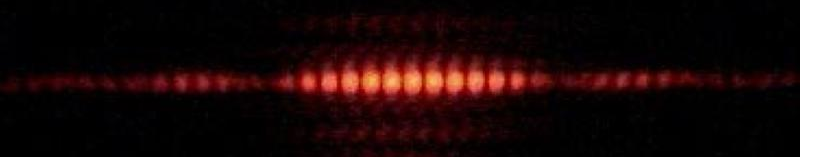
\includegraphics[scale=0.175,angle=90]{figures/Waves/fringes}};
%\clip (\w/2,-\d/2-\gap-\h) rectangle (\w/2+0.1,\d/2+\gap+\h);

}
\end{tikzpicture}
\captionof*{figure}{\textit{The interference pattern from light shining through two slits (double-slit experiment).}}
\end{center}
}
{
\capfig{1}{figures/Waves/veritassium}{Veritasium (former Queen’s student!). Waves are created by two ball oscillating on top of the water. \url{https://www.youtube.com/watch?v=Iuv6hY6zsd0}}
}


%%%%%%%%%%%%%%%%%%%%%%%%%%%%%%%%
\subsubsection{Waves from two sources}
\label{subsubsec:wavesfromtwosources}
\begin{frame}{Waves from two sources}
\begin{center}
\animategraphics[autoplay,loop,width=10cm]{10}{figures/Waves/vwaves-}{0}{71}
\end{center}
https://www.youtube.com/watch?v=Iuv6hY6zsd0
\end{frame}


%%%%%%%%%%%%%%%%%%%%%%%%%%%%%%%%
\begin{frame}{Speakers interfering and beats}
\begin{center}

\begin{animateinline}[autoplay,loop]{10} % 5 fps, same as 0.2 s transduration

\multiframe{24}{i=1+1}{

\begin{tikzpicture}[scale=1]
\tikzmath{
\L=10;
\h=0.7;
\Ax1=0.75*\h;
\wl1=\L/40;%wavelength
\om1=2*pi/\wl1;%effective frequency
\Ax2=\Ax1;
\om2=1.05*\om1;%effective frequency
\phas=-2*pi/24*\i;
}
\scalebox{1}{

\draw[-latex,line width=1] (0,-\h) -- (0,1.2*\h) node[left]{$D_1$};
\draw[-latex,line width=1] (0,0) -- (1.05*\L,0) node[below]{$x$};

\draw[color=black!50] (0,-\h) grid[step=0.25] (\L,\h);
\draw[trig format=rad, line width=1,color=myblue!60] plot[ domain=0:\L, variable=\x, samples=700] ({\x},{\Ax1*sin(\om1*\x+\phas)});

\begin{scope}[shift={(0,-2.2*\h)}]
\draw[-latex,line width=1] (0,-\h) -- (0,1.2*\h) node[left]{$D_2$};
\draw[-latex,line width=1] (0,0) -- (1.05*\L,0) node[below]{$x$};
\draw[color=black!50] (0,-\h) grid[step=0.25] (\L,\h);
\draw[trig format=rad, line width=1,color=myblue!60] plot[ domain=0:\L, variable=\x, samples=700] ({\x},{\Ax2*sin(\om2*\x+\phas)});
\end{scope}

\begin{scope}[shift={(0,-5.9*\h)}]
\draw[-latex,line width=1] (0,-2.1*\h) -- (0,2.3*\h) node[left]{$D$};
\draw[-latex,line width=1] (0,0) -- (1.05*\L,0) node[below]{$x$};
\draw[color=black!50] (0,-2.1*\h) grid[step=0.25] (\L,2.1*\h);
\draw[trig format=rad, line width=1,color=myred] plot[ domain=0:\L, variable=\x, samples=700] ({\x},{\Ax1*sin(\om1*\x+\phas)+ \Ax2*sin(\om2*\x+\phas)});
\end{scope}

}
\end{tikzpicture}
}
\end{animateinline}
\captionof*{figure}{\textit{Waves with slightly different frequencies result in ``beats'' (here the frequencies are different by 5\%).}}
\end{center}
\end{frame}


%%%%%%%%%%%%%%%%%%%%%%%%%%%%%%%%
\subsection{Standing waves}
\label{subsec:standingwaves}
\begin{frame}{Standing waves}
\begin{itemize}
\item Particles in the medium are oscillating, but energy is not moving through the medium (as opposed to traveling waves).
\item This happens when waves traveling in opposite directions interfere, usually with their own reflections.
\item Examples:
\begin{itemize}
\item Vibrating guitar/piano/violin string.
\item Vibrating air inside an organ pipe.
\end{itemize}
\end{itemize}
\end{frame}


%%%%%%%%%%%%%%%%%%%%%%%%%%%%%%%%
\begin{frame}{Standing waves}
\begin{center}

\begin{animateinline}[autoplay,loop]{10} % 5 fps, same as 0.2 s transduration

\multiframe{48}{i=1+1}{

\begin{tikzpicture}[scale=1]
\tikzmath{
\L=8;
\h=0.7;
\Ax=0.75*\h;
\wl1=\L/6;%wavelength
\om1=2*pi/\wl1;%effective frequency
\phas=-2*pi/48*\i;
}
\scalebox{1}{

\useasboundingbox (-\L/4,-2.2*\Ax) rectangle (5*\L/4,2.2*\Ax);
\draw[trig format=rad, line width=1, color=myblue!60] plot[domain=0:5*\L/4, variable=\x, samples=100] ({\x},{\Ax*sin(\om1*\x-\phas)});
\draw[trig format=rad, line width=1, color=myblue!60] plot[domain=-\L/4:\L, variable=\x, samples=100] ({\x},{\Ax*sin(\om1*\x+\phas)});
\draw[trig format=rad, line width=1.5, color=myred] plot[domain=0:\L, variable=\x, samples=100] ({\x},{\Ax*sin(\om1*\x-\phas)+\Ax*sin(\om1*\x+\phas)});

}
\end{tikzpicture}
}
\end{animateinline}
\captionof*{figure}{\textit{Two traveling waves interfering to make a standing wave.}}
\end{center}



\begin{center}

\begin{animateinline}[autoplay,loop]{10} % 5 fps, same as 0.2 s transduration

\multiframe{48}{i=1+1}{

\begin{tikzpicture}[scale=1]
\tikzmath{
\L=8;
\h=0.7;
\Ax=0.75*\h;
\wl1=\L/3;%wavelength
\om1=2*pi/\wl1;%effective frequency
\phas=-2*pi/48*\i;
}
\scalebox{1}{

\useasboundingbox (-\L/4,-2.2*\Ax) rectangle (5*\L/4,2.2*\Ax);
\draw[trig format=rad, line width=1, color=myblue!60] plot[domain=0:5*\L/4, variable=\x, samples=100] ({\x},{\Ax*sin(\om1*\x-\phas)});
\draw[trig format=rad, line width=1, color=myblue!60] plot[domain=-\L/4:\L, variable=\x, samples=100] ({\x},{\Ax*sin(\om1*\x+\phas)});
\draw[trig format=rad, line width=1.5, color=myred] plot[domain=0:\L, variable=\x, samples=100] ({\x},{\Ax*sin(\om1*\x-\phas)+\Ax*sin(\om1*\x+\phas)});

}
\end{tikzpicture}
}
\end{animateinline}
\captionof*{figure}{\textit{Two different traveling waves interfering to make a standing wave.}}
\end{center}

\end{frame}

%%%%%%%%%%%%%%%%%%%%%%%%%%%%%%%%

%%%%%%%%%%%%%%%%%%%%%%%%%%%%%%%%
\subsubsection{Fundamentals and harmonics}
\label{subsubsec:fundamentalsandharmonics}
\twocolframesf{Standing waves: fundamentals and harmonics}
{
\begin{itemize}
\item We can characterize a standing wave by the number of nodes (don't move) and anti-nodes (max amplitude).
\item For a standing wave on a string, the ends are always nodes.
\end{itemize}
}
{
\begin{center}
\begin{tikzpicture}[scale=1]
\tikzmath{
\h=1.25;
\w=0.2;
\L=4;
\Ax=0.45*\h;
\wl1=2*\L;%wavelength
\om1=2*pi/\wl1;%effective frequency
\wl2=\L;
\om2=2*pi/\wl2;%effective frequency
\wl3=2*\L/3;
\om3=2*pi/\wl3;%effective frequency
}
\scalebox{1}{

\fill[color=myblue!60] (\L,-\h/2) rectangle +(\w,\h);
\node at (0,0) {
\includegraphics[scale=0.05,angle=-90]{figures/Waves/hand}};
\draw[dashed,brown,line width=1.5] (0,0) -- (\L,0);
\draw[trig format=rad, line width=1.5, color=brown] plot[ domain=0:\L, variable=\x, samples=100] ({\x},{\Ax*sin(\om1*\x)});
\draw[trig format=rad, line width=1.5, color=brown,dashed] plot[ domain=0:\L, variable=\x, samples=100] ({\x},{-\Ax*sin(\om1*\x)});

\begin{scope}[shift={(0,-1.1*\h)}]
\fill[color=myblue!60] (\L,-\h/2) rectangle +(\w,\h);
\node at (0,0) {
\includegraphics[scale=0.05,angle=-90]{figures/Waves/hand}};
\draw[dashed,brown,line width=1.5] (0,0) -- (\L,0);
\draw[trig format=rad, line width=1.5, color=brown] plot[ domain=0:\L, variable=\x, samples=100] ({\x},{\Ax*sin(\om2*\x)});
\draw[trig format=rad, line width=1.5, color=brown,dashed] plot[ domain=0:\L, variable=\x, samples=100] ({\x},{-\Ax*sin(\om2*\x)});
\end{scope}

\begin{scope}[shift={(0,-2.2*\h)}]
\fill[color=myblue!60] (\L,-\h/2) rectangle +(\w,\h);
\node at (0,0) {
\includegraphics[scale=0.05,angle=-90]{figures/Waves/hand}};
\draw[dashed,brown,line width=1.5] (0,0) -- (\L,0);
\draw[trig format=rad, line width=1.5, color=brown] plot[ domain=0:\L, variable=\x, samples=100] ({\x},{\Ax*sin(\om3*\x)});
\draw[trig format=rad, line width=1.5, color=brown,dashed] plot[ domain=0:\L, variable=\x, samples=100] ({\x},{-\Ax*sin(\om3*\x)});

\end{scope}


}
\end{tikzpicture}
\captionof*{figure}{\textit{The first 3 harmonics (fundamental, first overtone, second overtone).}}
\end{center}
}


%%%%%%%%%%%%%%%%%%%%%%%%%%%%%%%%
\subsubsection{Resonance}
\label{subsubsec:resonance}
\begin{frame}{Standing waves and resonance}
\begin{itemize}
\item We can think of objects as having ``resonant frequencies'' that correspond to the frequencies (wavelengths) of the fundamental frequency and the harmonics.
\item If you make an object vibrate, most of the waves will destructively interfere, but the waves at the right frequencies can setup standing waves that can become quite large. 
\item You don't need to shake the end of the object at a particular frequency to create a standing wave inside of it. 
\item If you pluck a guitar string, you effectively send a bunch of sine waves along the string; those that correspond to the harmonics will constructively interfere and dominate the sound that you hear.
\end{itemize}
\end{frame}


%%%%%%%%%%%%%%%%%%%%%%%%%%%%%%%%



%%%%%%%%%%%%%%%%%%%%%%%%%%%%%%%%


%%%%%%%%%%%%%%%%%%%%%%%%%%%%%%%%


%%%%%%%%%%%%%%%%%%%%%%%%%%%%%%%%
\twocolframe{Description of a standing wave}
{
\begin{itemize}
\item In contrast to a traveling wave, in a standing wave, each point oscillates with a different amplitude.
\item We can describe each point on the string with:
\begin{align*}
D(x,t)=2A\sin\left(\frac{n\pi}{L}x\right) \cos(\omega t)
\end{align*}
\item Each point oscillates as a simple harmonic oscillator:
\begin{align*}
D(x,t)=A(x)\cos(\omega t)
\end{align*}
\end{itemize}
}
{
\begin{center}
\begin{tikzpicture}[scale=1]
\tikzmath{
\h=1.25;
\w=0.2;
\L=4;
\Ax=0.45*\h;
\wl1=2*\L;%wavelength
\om1=2*pi/\wl1;%effective frequency
\wl2=\L;
\om2=2*pi/\wl2;%effective frequency
\wl3=2*\L/3;
\om3=2*pi/\wl3;%effective frequency
}
\scalebox{1}{

\fill[color=myblue!60] (\L,-\h/2) rectangle +(\w,\h);
\node at (0,0) {
\includegraphics[scale=0.05,angle=-90]{figures/Waves/hand}};
\draw[dashed,brown,line width=1.5] (0,0) -- (\L,0);
\draw[trig format=rad, line width=1.5, color=brown] plot[ domain=0:\L, variable=\x, samples=100] ({\x},{\Ax*sin(\om1*\x)});
\draw[trig format=rad, line width=1.5, color=brown,dashed] plot[ domain=0:\L, variable=\x, samples=100] ({\x},{-\Ax*sin(\om1*\x)});

\begin{scope}[shift={(0,-1.1*\h)}]
\fill[color=myblue!60] (\L,-\h/2) rectangle +(\w,\h);
\node at (0,0) {
\includegraphics[scale=0.05,angle=-90]{figures/Waves/hand}};
\draw[dashed,brown,line width=1.5] (0,0) -- (\L,0);
\draw[trig format=rad, line width=1.5, color=brown] plot[ domain=0:\L, variable=\x, samples=100] ({\x},{\Ax*sin(\om2*\x)});
\draw[trig format=rad, line width=1.5, color=brown,dashed] plot[ domain=0:\L, variable=\x, samples=100] ({\x},{-\Ax*sin(\om2*\x)});
\end{scope}

\begin{scope}[shift={(0,-2.2*\h)}]
\fill[color=myblue!60] (\L,-\h/2) rectangle +(\w,\h);
\node at (0,0) {
\includegraphics[scale=0.05,angle=-90]{figures/Waves/hand}};
\draw[dashed,brown,line width=1.5] (0,0) -- (\L,0);
\draw[trig format=rad, line width=1.5, color=brown] plot[ domain=0:\L, variable=\x, samples=100] ({\x},{\Ax*sin(\om3*\x)});
\draw[trig format=rad, line width=1.5, color=brown,dashed] plot[ domain=0:\L, variable=\x, samples=100] ({\x},{-\Ax*sin(\om3*\x)});

\end{scope}


}
\end{tikzpicture}
\captionof*{figure}{\textit{The first 3 harmonics (fundamental, first overtone, second overtone).}}
\end{center}
}

%%%%%%%%%%%%%%%%%%%%%%%%%%%%%%%%



%%%%%%%%%%%%%%%%%%%%%%%%%%%%%%%%



%%%%%%%%%%%%%%%%%%%%%%%%%%%%%%%%



%%%%%%%%%%%%%%%%%%%%%%%%%%%%%%%%



%%%%%%%%%%%%%%%%%%%%%%%%%%%%%%%%



%%%%%%%%%%%%%%%%%%%%%%%%%%%%%%%%



%%%%%%%%%%%%%%%%%%%%%%%%%%%%%%%%



%%%%%%%%%%%%%%%%%%%%%%%%%%%%%%%%



%%%%%%%%%%%%%%%%%%%%%%%%%%%%%%%%



%%%%%%%%%%%%%%%%%%%%%%%%%%%%%%%%



%%%%%%%%%%%%%%%%%%%%%%%%%%%%%%%%



%%%%%%%%%%%%%%%%%%%%%%%%%%%%%%%%



%%%%%%%%%%%%%%%%%%%%%%%%%%%%%%%%



%%%%%%%%%%%%%%%%%%%%%%%%%%%%%%%%






\end{document}
\begin{frame}{test}

\end{frame}

